{\Huge\textbf{ DELETE THIS PAGE}}
\section{Poznámky - informačný účel}
Táto strana slúži na poznámky, TODO, toho čo mám ešte urobiť. 
Bude samozrejme zmazaná.  
Dany text, ktory sa bude dat pouzit v praci bude presunuti do jadra prace. 

dopnit do praktickej casti mapu: vyuzivajuc tento priklad ovladania.. \url{http://raphaeljsvectorgraphics.com/the-graphical-web/turtle-graphics-logo}
pozriet si funkciu snap - inAnim()...


Pridat postup ako sa ziska Snap zo stranky a implementuje do html dokumentu. .

ujednotnit nazov attribut a parameter

\section{Kapitoly by mali byt nasledovne}
\begin{enumerate}
	\item ciel prace 
	\item metodika prace
	\item definovanie zakladnych pojmov / co je html5, co je scada system, a co je svg vektorova grafika (takmer hotove, len nemam scada systemy definovane), 
	\item analyza nastrojov - preco som sa rozhodla pouzit inkscape na tvorbu svg obrazkov, //este tam musim spomenut moznost exportu do formatov... 
	\item postup na vytvorenie OBRAZKA SVG V INKSCAPE
	\item priklad vytvorenia precepavacej stanice v Inkscape (toto je uz takmer hotove)
	\item ANALYZA javascriptovych kniznic / (toto uz je takmer hotove, este tam pridat jquery )
	\item Postup \textbf{tvorby} grafickych komponentov cez Snap... 
	\item Postup \textbf{animacie} uz vytvorenych grafickych elementov 
	\item Priklad v kode animovanie Precerpavaciej stanice... (Takmer hotove) toto je vlastne ta implementacia vzorovej sady grafickych komponentov
	\item Navrh REST API na prepojenie grafickych komponentov so SCADA SERVEROM  \textit{toto no nemam / mam iba priklad kodu jednoducheho }
	\item Analyza moznosti automatickeho mapovania api grafickych prvkov pomocou metadat na existujuce api dostupne pre scada serverr D2000 \textit{tooto nemam vobec}
	\item analyza vykonnosti a vykonnostne obmedzenia - toto iba okrajovo spomeniem - vseobecne preco je lepsie svg, a preco nie je vhodne, v prvej kapitole som pisala rozdiel medzi canvas a svg - istym sposobom to je analyza obmedzeni.. ?
	\item zhrnutie
	
\end{enumerate}


\newpage
\section{Learning Raphael JS Vector Graphics}
%V práci cituj: \cite{Dawber} , strany sa cituju takto: \cite[p.~215]{Dawber} \\ Priklady z knihy:\url{http://raphaeljsvectorgraphics.com/}  \cite{Dawber} .
%Z tejto knihy idem pridávať do bakalárky nasledovné veci:
%Namet na zmenu: pouzit to demo, ktore mi poslal veduci na transformaciu zmeny. 


\section{Porovnanie spôsobu vykreslenia cez \acs{SVG} \acs{SMIL} a Snap}

Kreslenie vektorov je jednoduchšie cez Snap ako čisto písanie SVG. 

Príklad kreslenia obdĺžníka a animovanie šírky z 50 pixlov na 100 pixelov cez SVG SMIL:\cite[p.~9]{Dawber}
\begin{lstlisting}
<svg>
<rect x="10" y="10" width="50" height="30">
	<animate attributeType="XML"
		attributeName="width"
		to="100"
		fill="freeze"
		dur="10s"  />
</rect></svg>
\end{lstlisting}

Nakreslíme obdĺžnik na súradniciach (10, 10) s šírkou 50, a výškou 30 použitím elementu $<$rect$>$. Zoskupený element $<$animate$>$ definuje animáciu zmeny šírky obdĺžnika na šírku 100 px, ktorá trvá desať sekúnd. Kde fill="freeze" je použité na zachovanie stavu obdĺžnika po ukončení animácie. Inak by bola nastavená na 50. 

Ekvivalent k animácii cez Snap API v nasledujúcom príklade:

\begin{lstlisting}
paper = Snap();
var rect = paper.rect(10, 10, 50, 30);
rect.animate({
	width: 100
	}, 10000);
\end{lstlisting}

Syntax metód animate a rect je výstižnejšia a lepšia na pochopenie. Snap sa tiež dobre integruje s inými knižnicami, ako napríklad jQuery. 


%%%%%%%%%%%%%%%%%%%%%%%%%%%%%%%%%%%%%%%%%%%%%%%%%%%%%%%%%%%%%%%%%%%%%%%%%%%%%%%%%%%%%%%%%%%%%%%%%%%%%%%%%%%%%%%%%%%%%%%%%%%%%%%%%%%%%%%%%%%%%%%%%%%%%%%%%%%%%%%%%%%%%%%%%%%%%%%%%%%%%%%%%%%%%%%%%%%%%%%%%%%%%%%%%%
\newpage
%Jednoduche kreslenie ,
%Interakcia ,
%Animovanie.. 
%
%Krok 0: ziskanie Snapu...

 
\section{Krok 1: Inicializácia plátna na kreslenie}
%viewport = výrez
Na to, aby sme boli schopní kresliť grafické komponenty, tak potrebujeme definovať miesto, kde budú vykreslené. 
%Určenie miesta, kde bude vykreslené plátno je buď viditeľné okno vo webovom prehliadači, alebo viewport. 
Viditeľná oblasť okna prehliadača, alebo viewport, definuje oblasť, v ktorej sa vykreslí komponent na plátno.
SVG špecifikácia referuje ako miesto vykreslenia seba ako viewport. 
Inak povedané viewport je akákoľvek obdĺžniková oblasť.
Okno prehliadača je referencia na viewport a kresliaca oblasť je plátno.   \cite{Dawber}


Vytvorenie plátna cez Snap konštruktor sa dá urobiť viacerými spôsobmi.

\subsection{Súradnice plátna}
 
 
Nasledujúci príkaz zadefinuje pláno s rozmermi šírka je 300 a výška 200. 
\begin{lstlisting}
var paper = Snap(300, 200);
\end{lstlisting}


Na obrázku \ref{fig:suradnice1}  je znázornená východzí súradnicový systém plátna vytvoreného cez Snap konštruktor. 
Začiatok súradnic na osi x, y je rovné nule. Bod na plátne so súradnicami x = 300, y = 200 alebo (300, 200) vo vektorovom zápisu je bod 300px vpravo od začiatku x-ovej osi a 200px dole od počiatku y-ovej osi. 

\begin{center}
	\begin{figure}[hp]
\centering
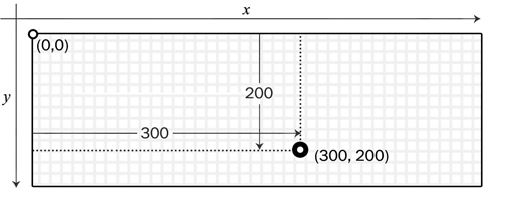
\includegraphics[width=0.7\linewidth]{obrazky/suradnice1}
\caption{Súradnicový systém plátna s bodom (300, 200)}
\label{fig:suradnice1}
\end{figure}
\end{center}


\subsection{DOM element}

Dosť často je potrebné použiť existujúci DOM element ako kontajner pre plátno než viewport. Ako element môžeme použiť napríklad:
\begin{lstlisting}
 <div id="mojePlatno"></div>  
 \end{lstlisting}

Nasledujúcim kódom vytvorím 500px široké a 300px vysoké plátno.

\begin{lstlisting}
var paper = Snap("mojePlatno", 500, 300);
\end{lstlisting}

Keď využívam túto formu konštruktora, tak prvý element je ID elementu. Alternatívne sa dá prvý parameter DOM element napísať nasledovným spôsobom: 
\begin{lstlisting}
Snap(document.getElementById('mojePlatno'), 500, 300);
\end{lstlisting}



\subsubsection{\acs*{SVG} v HTML dokumente}

SVG môže byť zobrazená buď ako inline v HTML dokumente, alebo ako vloženým samostatného .SVG súboru. 
V tabuľke \ref{vytvorenie:SVG} sú vymenované HTML tagy na zobrazenie SVG. 


\begin{table}[hp]
	\begin{center}
		\begin{tabular}{|l|l|}
			\hline \textbf{Technika} & \textbf{Popis} \\ 
			\hline
			\hline $<$embed$>$ tag & Načíta vytvorený SVG súbor.  \\ 
			\hline $<$object$>$ tag & Nepovoľuje skriptovanie.  \\ 
			\hline $<$iframe$>$ tag & Zobrazí SVG v rámci  \\ 
			\hline Inline $<$svg$>$ tag & Vytvorí Svg  \\ 
			\hline 
		\end{tabular} 
	\end{center}
	\caption{Spôsoby vytvorenia SVG v HTML dokumente}
	\label{vytvorenie:SVG}
\end{table}


%Príklady načítania SVG v HTML dokumente:
%\begin{itemize}
%\item Image 	
%\begin{lstlisting}
%<img src="stanica2.svg" width = "50" height= "50" />
%\end{lstlisting}
%\item Embed
%\begin{lstlisting}
%<embed src="stanica2.svg" width = "50" height= "50" />
%\end{lstlisting}
%\item Objekt
%\begin{lstlisting}
%<object type="image/svg+xml" data="stanica2.svg"
%width="50" height="50"></object>
%\end{lstlisting}
%\item IFrame
%\begin{lstlisting}
%<iframe src="stanica2.svg" width = "50" height= "50">
%</iframe>
%\end{lstlisting}
%\item Inline
%\begin{lstlisting}
%<svg width="100" height="100"> 
%<circle cx="50" cy="50" r="40"/> </svg>
%\end{lstlisting}
%	
%
%\end{itemize}





%%%%%%%%%%%%%%%%%%%%%%%%%%%%%%%%%%%%%%%%%%%%%%%%%%%%%%%%%%%%%%%%%%%%%%%%%%%%%%%%%%%%%%%%%%%%%%%%%%%%%%%%%%%%%%%%%%%%%%%%%%%%%%%%%%%%%%%%%%%%%%%%%%%%%%%%%%%%%%%%%%%%%%%%%%%%%%%%%%%%%%%%%%%%%%%%%%%%%%%%%%%%%%%%%%%%%%%%%
\newpage

\section{Kreslenie základných tvarov cez Snap}

Snap API poskytuje metódy na kreslenie jednoduchých tvarov. 

\begin{table}[hp]
	\begin{center}
		\begin{tabular}{|l|l|l|l|}
		\hline \textbf{Tvar} & \textbf{SVG element} & \textbf{Snap metoda} & \textbf{Atribúty} \\ 
		\hline Obdlžnik & $<$rect$>$ & .rect() & x, y, šírka, výška, rx, ry \\ 
		\hline Kruh & $<$circle$>$ & .circle() & r, x, y, cx, cy, rx, ry \\ 
		\hline Elipsa & $<$ellipse $>$ & .ellipse() & x, y, cx, cy, rx, ry \\ 
		\hline Čiara & $<$line$>$ & .line() & x1, y1, x2, y2 \\ 
		\hline Polyline & $<$polyline$>$ & .polyline() & pole x, y suradnic bodov \\ 
		\hline Polygon & $<$polygon$>$ & .polygone() & pole x, y suradnic bodov \\ 
		\hline Path & $<$path$>$ & .path() & vid tabuľka \ref{prikazy:Path}  \\ 
		\hline 
	\end{tabular} 
	
	\end{center}
	
	\label{porovnanieSVG:Snap}
	\caption{Zoznam tvarov, ktoré podporuje SVG a Snap API, a TODO TODO POROZMYSLAT NAD NAZVOM a atributy pre definovanie tvaru}
\end{table}




Tvar, ktorý je vykreslený cez Snap API má nasledovnú syntax: 

\begin{lstlisting}
	var paper = Snap(...);
	var tvar = paper.NazovSnapMetody({
			nazovAtributu: "hodnotaAtributu",
			 ...
			});
\end{lstlisting}

Tvar, ktorý je vykreslený priamo na HTML webovej stránke má vo vnútri elementu $<$svg$>$ definované atribúty nasledujúcim spôsobom: 

\begin{lstlisting}
	<ElementTvar nazovAtributu = "hodnotaAtributu" ... />
\end{lstlisting}


\subsection{Popis atribútov tvarov}

Názvy atribútov a ich význam pre obdĺžnik, kruh, elipsu sú vyjadrené v tabuľke \ref{parametre:tvar} 

\begin{table}[tp]
	\begin{center}
		\begin{tabular}{|l|l|}
			\hline \textbf{Parameter} & \textbf{Poznámka} \\ 
			\hline
			\hline x, y & súradnica x-osi, y-osi  \\ 
			
			\hline cx & x-os súradnica centra kruhu, alebo elipsy \\ 
			\hline cy & y-os súradnica centra kruhu, alebo elipsy \\ 
			\hline r & polomer kruhu, elipsy alebo okruhlých rohov na obdĺžniku \\ 
			\hline rx & horizontálny polomer elipsy \\ 
			\hline ry & vertikálny polomer elipsy \\ 
			\hline x1, y1 & začiatočné x, y súradnice \\
			\hline x2, y2 & konečné x, y súradnice \\
			
			%\hline width, height & šírka, výška\\
			\hline
		\end{tabular} 
		
	\end{center}
	\caption{Názvy atribútov a ich význam}
	\label{parametre:tvar}
\end{table}

Pre útvary polyline, polygon sú atribúty dvojice súradníc osi x, y, ktoré určujú body, ktoré sa spoja. 



\subsubsection{Path tvar}


V Snap API je to metóda Paper.path([pathString]), ktorá vytvorí $<$path$>$ element podľa daného reťazca.  Parameter pathString pozostáva reťazca skladajúceho sa z jedno písmenkových príkazov, nasledovanými bodkami a oddeľovaný argumentami a číslami. Príkazy sú uvedené v tabuľke \ref{prikazy:Path}.

Napríklad: "M10,20L30,40" - obsahuje príkazy: M s argumentami (10, 20) a L (30, 40). Rozdiel vo veľkosti písma vyjadruje to, či ide o absolútnu, alebo relatívnu cestu. Ak sú malé znaky jedná sa o relatívne, v prípade veľkých znakov absolútna cesta. 


\begin{center}
	\begin{table}[hp]
		\begin{center}
			\begin{tabular}{|c|l|c|}
				\hline \textbf{Príkaz} & \textbf{Názov} & \textbf{Parametre} \\
				\hline
				\hline M & moveto & (x y)+ \\ 
				\hline Z & closepath & (none) \\ 
				\hline L & lineto & (x y)+ \\ 
				\hline H & horizonal lineto & x+ \\ 
				\hline V & vertical lineto & y+ \\ 
				\hline C & curveto & (x1 y1 x2 y2 x y)+ \\ 
				\hline S & smooth curveto & (x2 y2 x y)+ \\ 
				\hline Q & quadratic Bézier curveto & (x1 y1 x y)+ \\ 
				\hline T & smooth quadratic Bézier curveto & (x y)+ \\ 
				\hline 
			\end{tabular} 
		\end{center}
		\caption{Niekoľko príkazov na tvorbu Path elementu}
		\label{prikazy:Path}
	\end{table}
\end{center}






\newpage
\clearpage
TOTO BUDE PRIKLAD KED BUDEM MAT UZ NAPISANE ATTRIBUTY NA ZMENU STYLU

\subsubsection{PRIKLAD TVORBY KRUHU A NASTAVENIE ATRIBUTOV }

Kód vytvoreného kruhu: 

\begin{lstlisting}
<svg width="100" height="100">
<circle cx="50" cy="50" r="40" stroke="black" stroke-width="2" fill="silver" />
</svg>	
\end{lstlisting}

SVG obrázok začína s $<$svg$>$ elementom. Atribúty elementu $<$svg$>$ sú width a height. Definujú šírku a výšku SVG obrázka. Element $<$circle$>$ je použitý na nakreslenie kruhu.


TODO TODO TODO

 Atribúty stroke a stroke-width určujú to ako bude vyzerať obrys útvaru. Kruh má nastavený 2px čierny okraj. 
Atribút fill vyplní vnútro kruhu. V príklade je vyplnený sivou farbou. Tag, ktorý uzavrie SVG obrázok je $<$$/$svg$>$. Keďže SVG je validné XML, tak všetky elementy musia byť správne zatvorené. \cite{inline}

Kruh vytvorený cez Snap API má nasledovný kód:

\begin{lstlisting}
var paper = Snap(100, 100);
var kruh = paper.circle(50, 50, 40);
	kruh.attr({
	stroke: "black", 
	strokeWidth: 2, 
	fill: "silver"
});

\end{lstlisting}


Vykreslí sa na HTML stránku obrázok \ref{jednoduchyKruh}. Obidva spôsoby vykreslili kruh na webovej stránke úplne rovnako.  
 
 \begin{figure}[hp]
 	\begin{center}
 		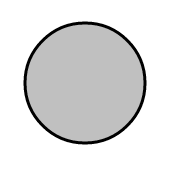
\includegraphics  {obrazky/jednoduchyKruh.png}
 		\caption{Vykreslený kruh vytvorený cez SVG, a Snap API}
 		\label{jednoduchyKruh}
 	\end{center}
 \end{figure}









